\chapter*{John the Baptist}

Let us return now to the very beginning of Jesus Christ's public ministry, when fate brought him face-to-face with the last of the Old Testament prophets, John the Baptist. The Forerunner of the Savior (``He who is coming after me is mightier than I''---Mt 3:11), who considered himself ``not worthy to loose His sandal strap'' (Jn 1:27), John was the first to correctly recognize the divine essence of Jesus: ``Behold! The Lamb of God who takes away the sin of the world!'' (Jn 1:29). A man who sharply rebuked both religious and secular leaders (``Brood of vipers! Who warned you to flee from the wrath to come?''---Mt 3:7), he paid with his life for his denunciation of the lawlessness and debauchery that Herod, the tetrarch of Galilee, was mired in. At first glance, this personage (whose historicity, incidentally, is without question) seems to have absolutely no mystery about him. However, let us conduct a careful and impartial analysis of John's relationships---first, with Jesus, and second, with the authorities (in particular, Herod Antipas).

The first (and last) meeting between Jesus and John took place on the banks of the River Jordan, in whose waters the prophet would baptize the crowds of people who flocked to him. Jesus, among others, asked to be baptized; John ``would have prevented him, saying, `I need to be baptized by You, and are You coming to me?''' (Mt 3:14). The moment the ritual was performed, the Holy Spirit descended upon Jesus in the form of a dove (visible only to the Baptist, however). The episode of the baptism is described practically identically by all four Evangelists, but afterwards, like usual, significant discrepancies begin to emerge between John and the Synoptists.

John the Evangelist writes that the next day, John the Baptist sent Jesus adetachment of two of his own novices---Andrew and another not mentioned by name---who became his first disciples. Later on, Jesus and his newly formed community returned to Galilee, where he performed his first miracles. Then, he went on his first Passover pilgrimage to Jerusalem; there, he expelled the money changers from the Temple for the first time, and also held a nighttime conversation with a member of the Sanhedrin named Nicodemus. After this:

\begin{smallquote}
    Jesus and his disciples came into the land of Judea, and there He remained with them and baptized. Now John also was baptizing in Aenon near Salim, [...] \emph{for John had not yet been thrown into prison}'' (Jn 3:22-24).
\end{smallquote}
Let's keep this last phrase in the back of our minds; it is very important.

Since by this point, more people were coming to Jesus to get baptized than
to John, the latter's disciples voiced their resentment at the success of their ``rival." John, however, admonished them for their jealousy, comparing Jesus to a bridegroom, and himself to the best man, who must not envy his friend, but feel happy for him (``He must increase, but I must decrease''---Jn 3:30). Following this, all references to John the Baptist in the Gospel of John disappear.

Now, let us return to the phrase ``for John had not yet been thrown into prison.'' Given that it appears in the chronologically last of the four Gospels, it comes across as a direct objection to the Synoptists' version, and an attempt to remind them of how things really were. After all, if you believe the Synoptists, Jesus retreated into the desert immediately after his baptism to pray and overcome temptation; it was there that he learned of John's arrest (Mt 4:12, Mk 1:14). Only \emph{after} he received this news did he travel to Galilee, and only \emph{there} did he gain his first disciples, Andrew and Simon---fishermen on the Sea of Galilee. The importance of this seemingly insignificant detail---when precisely the Baptist was arrested---becomes clear from the subsequent narrative of the Sypnotists

Matthew and Luke go on to recount the so-called ``Embassy from John the Baptist''; after hearing of the miracles Jesus has performed, the prophet sends two of his disciples to him to investigate:

\begin{smallquote}
    ``Are You the Coming One, or do we look for another?'' Jesus answered and said to them, ``Go and tell John the things which you hear and see: The blind see and the lame walk; the lepers are cleansed and the deaf hear; the dead are raised up and the poor have the gospel preached to them.'' (Mt 11:3-5)
\end{smallquote}
After John's disciples depart, Jesus delivers a panegyric in honor of his Forerunner:

\begin{smallquote}
    ``Assuredly, I say to you, among those born of women there has not risen one greater than John the Baptist. [...] And if you are willing to receive it, he is Elijah who is to come'' (Mt 11:11-14).
\end{smallquote}

When you really think about it, this episode contradicts the entirety of the
narrative preceding it. It's bad enough that the \emph{Forerunner} is continuing his
ministry alongside the Lamb of God, who has \emph{already come} into this world. That
aside: if you have any grounds to believe that the Messiah has arrived, then surely
your first instinct would be to go see him yourself, and not send your disciples to
check things out. However, the Synoptists already have this question covered: the
only reason John the Baptist didn't come in person was because he was in prison at
the time (Mt 11:2), having been arrested almost immediately after Jesus' baptism.

But then John snaps back: nothing of the sort---the Baptist was still a free man for quite some time afterwards, and was performing baptisms side-by-side with Jesus. It seems the Evangelist understood the true meaning of this episode far better than the Synoptists did, for which reason he deliberately excluded it from his narrative---as this episode makes it abundantly clear that even in the best case scenario, the Forerunner had his doubts as to whether Jesus really was He who would ``baptize with the Holy Spirit and fire'' (Lk 3:16). What's more, the Synoptists are completely silent as to how John reacted to his ambassadors' report. If that's the case, then what to make of everything John said upon meeting him personally (``Lamb of God,'' ``you come to be baptized by me?''), or the sign given directly to John in the form of a dove? Incidentally, I should point out that the entire scene of the baptism (as well as John's subsequent ``exhortation on Christ''---Jn 3:22-36) is what is known in legal terms as ``hearsay,'' as none of the Evangelists were personally there to witness it.

If you objectively analyze everything John said (and even more so, did), you inevitably arrive at a discouraging conclusion: at no point did the Forerunner clearly and unequivocally recognize his distant relative (according to Luke) as He who ``would come after him more powerful than he.'' Several of the Baptist's statements regarding Jesus (for example, ``and no one receives His testimony''---Jn 3:32) have forced Christian commentators to resort to plaintive explanations such as, ``The Evangelist didn't quite accurately convey the prophet's meaning...'' If we so desired, we could easily read some episodes differently from the way they are typically interpreted.

Take, for example, how Gladkov describes the scene of the baptism:
\begin{smallquote}
    Recognizing that John had been sent by God to baptize, Jesus, a Man who had heretofore fulfilled all the Lord's commandments, began His ministry by fulfilling the last Old Testament commandment, which God had just announced through John. \emph{As He was without sin, He had no need to repent, for which reason he petitioned John directly to baptize Him} [emphasis mine---K.E.]. John saw at once that this was no ordinary man standing before him, and thus replied: ``I need to be baptized by you, and do you come to me?''
\end{smallquote}

Now here's how \emph{I} imagine this scene might have played out. Before this supremely authoritative prophet, who fills the Pharisees and Sadducees with awe and regularly sermonizes to enormous crowds of people, appears a young man who no one has ever seen before. He announces that since he is without sin, the only thing he needs from him is to be baptized. John, utterly astonished at such (from his perspective) insolence, throws up his hands with feigned humility. ``Guess you're right, buddy, you've come to the wrong guy. You know what, \emph{I} shouldn't be the one baptizing \emph{you}---\emph{you} should be the one baptizing \emph{me}!'' The audience is delighted---he sure showed him!

Christian commentators often claim that John himself directed his crowds of followers to Jesus; however, this is completely unsupported by the Gospel texts. It's possible some members of John's community actually did leave him for Jesus (Christ would go on to see many of his disciples leave him as well---a common occurrence), but this migration was clearly neither organized nor widespread. John the Evangelist's account of the Baptist ``gifting'' Jesus his first disciples, as we may recall, is unanimously contradicted by the Synoptists. A rather telling detail: after John's execution, his disciples made a special trip to tell Christ the news (Mt 14:12), but not one of them ended up joining his community!

The desire of John's disciples to stick by their teacher's side, especially during the trying times of his imprisonment, deserves nothing but respect. But then came John's demise; it would seem only natural for them to start following the man who their dearly beloved teacher (as the Evangelists tell us) deemed himself the forerunner to. Yet nothing of the sort ever happened. In fact, the Johannites maintain a separate identity from Christians to this very day, existing in the form of a Jewish sect; they have a ``Sacred Scripture'' of their own where John the Baptist is recognized as the Messiah, while Jesus is taken to be a false prophet. And when you really think about it, this is all perfectly natural. How do you think John---a somber, puritanical Jew---would take to a man who miraculously turned water into wine for partygoers and rubbed shoulders with prostitutes, tax collectors, and occasionally---perish the thought!---uncircumcised gentiles?

And so, we observe a rather pronounced asymmetry in opinion: for Christians, John is their greatest prophet and a highly revered figure in general, whereas for the Johannites, Jesus is a false messiah. In addition, there are no grounds to believe that each of these sects formed their opinions \emph{in spite of} the statements of their founders. For this reason, the Evangelists were faced with an intractable problem when it came time to describe these events. On the one hand, Jesus Christ, the Son of God, whose every word is Truth incarnate, had a very high opinion of John the Baptist (something they witnessed directly); on the other hand, said John, as far as they knew, did not return his feelings and was not particularly fond of their teacher. How could they possibly resolve such a contradiction?

Here's how: by taking the many statements of John the Baptist (both authentic ones and those attributed to him by rumor) and selecting only those that could point to him recognizing the divinity of the Evangelists' teacher. The lack of written texts made this task significantly easier. More likely than not, many of the statements attributed to John probably originated among Jesus' followers themselves. After circulating among the population at large (and gathering new ``details'' along the way), these stories later returned to the Evangelists, who gladly recorded them as ``independent testimony''---a well-known effect in sociology. The ``beloved disciple''---the author of the fourth gospel, John---went further down this path than the others did. Not only did he introduce the apocryphal episodes of Christ being ``gifted'' his first disciples and the ``exhortation on Christ'' (neither of which appear in the Synoptic Gospels), he also omitted such obvious kompromat as the mention of his teacher's ``inspection'' by the Baptist's disciples (which, on the contrary, he was certainly a witness to---along with the other Apostles).

So were the Evangelists deliberately trying to bolster their teacher's reputation by invoking the opinion of an authoritative independent source---modifying the latter's actual statements in order to suit their needs? No, no, and no! Any believer knows full well that Christ's authority---in the eyes of the Apostles---needed no ``independent testimony'' whatsoever to support it. For this reason, I am absolutely convinced that the Evangelists' correction of the Baptist's statements was a genuine attempt to save \emph{his} authority---the authority of a man who, for some reason, hesitated to recognize the patently obvious fact that Jesus was the Messiah. And needless to say, the Evangelists' efforts paid off; they literally created the John the Baptist who lives in our consciousness to this very day. The actual John, as I strongly suspect, would have justly occupied a place, if not alongside the Pharisees and other ``Jewish elders,'' then in any case very far away from the Son of Man.

Moving on to an analysis of John the Baptist's relationship with the secular authorities, we need to make one caveat. The Evangelists only knew the details of the prophet's tragic death through hearsay, just like any other citizen of Palestine who wasn't one of Herod's courtiers or a member of his secret police force. For this reason, the testimony of the New Testament texts will not be given any inherent precedence over that of Josephus' \emph{Antiquities}. Let us recall that \emph {Antiquities} is the only non-Christian source that directly mentions such figures from the Gospel as John the Baptist and James, the brother of Jesus. As a result, the Church treats Josephus' testimony with a high degree of reverence; in particular, it is from this source that the Baptist's place of captivity, the fortress of Machaerus,\footnote{``John the Baptist,'' Bible Encyclopedia, II:91-92.} is taken.

Mark the Evangelist (Mk 6:17-29) describes the prophet's death as follows. John, in spite of his imprisonment, continued to maintain his influence over Herod:

\begin{smallquote}
    Herod feared John, knowing that he was a just and holy man, and he protected him. And when he heard him, he did many things, and heard him gladly.
\end{smallquote}
The prophet, among other things, kept insisting that the tetrarch break off his relationship with Herodias, whom he married after divorcing his previous wife (the daughter of the Arab king Aretas IV) and dissolving the marriage of his brother Philip:
\begin{smallquote}
    Because John had said to Herod, ``It is not lawful for you to have your brother's wife.'' Therefore Herodias held it against him and wanted to kill him, but she could not.
\end{smallquote}

The opportunity presented itself at a feast, when Herodias' daughter Salome left Herod so stunned by her dancing that he quite simply went insane:

\begin{smallquote}
    He also swore to her, ``Whatever you ask me, I will give you, up to half my kingdom.''
\end{smallquote}
Uninterested in half of his kingdom, the princess, at her demonic mother's instigation, asked the king for the head of his irksome reproacher:

\begin{smallquote}
    And the king was exceedingly sorry; yet, because of the oaths and because of those who sat with him, he did not want to refuse her.
\end{smallquote}
One of his henchmen was dispatched to the prison, and several minutes later, he presented the bloodthirsty beauties a platter with the prophet's severed head. And small wonder: woman, of course, is the root of all evil, and truly is she said to be ``the devil's gateway''\footnote{Tertullian, \emph{On the Apparel of Women}, trans. Sydney Thelwall, Book 1, Chapter 1.} (and if you have any doubts, take another look at Oscar Wilde's \emph{Salome}).

Josephus, meanwhile, tells a different, far more prosaic story:

\begin{smallquote}
    Now when [many] others came in crowds about [John]; for they were very greatly moved [or pleased] by hearing his words; Herod, who feared lest the great influence John had over the people might put it into his power and inclination to raise rebellion... thought it best, by putting him to death, to prevent any mischief he might cause; and not bring himself into difficulties by sparing a man who might make him repent of it when it would be too late. Accordingly he was sent a prisoner, out of Herod's suspicious temper, to Macherus; the castle I before mentioned; and was there put to death. Now the Jews had an opinion, that the destruction of this army [in the war with Aretas] was sent as a punishment upon Herod; and a mark of God's displeasure to him.\footnote{\emph{Antiquities of the Jews}, Book XVIII, Chapter 5.}
\end{smallquote}
So, there were no personal motivations at work here---it was politics all the way down. In comparing these two versions, let us first turn to the factual side of the matter---specifically, everything we know about the marriage of Herod Antipas and Herodias.

% [htbp]: Instructs LaTeX to try placing the image Here, at the Top, Bottom, or on a separate Page (in that order).
\begin{figure}[htbp]
    \centering
    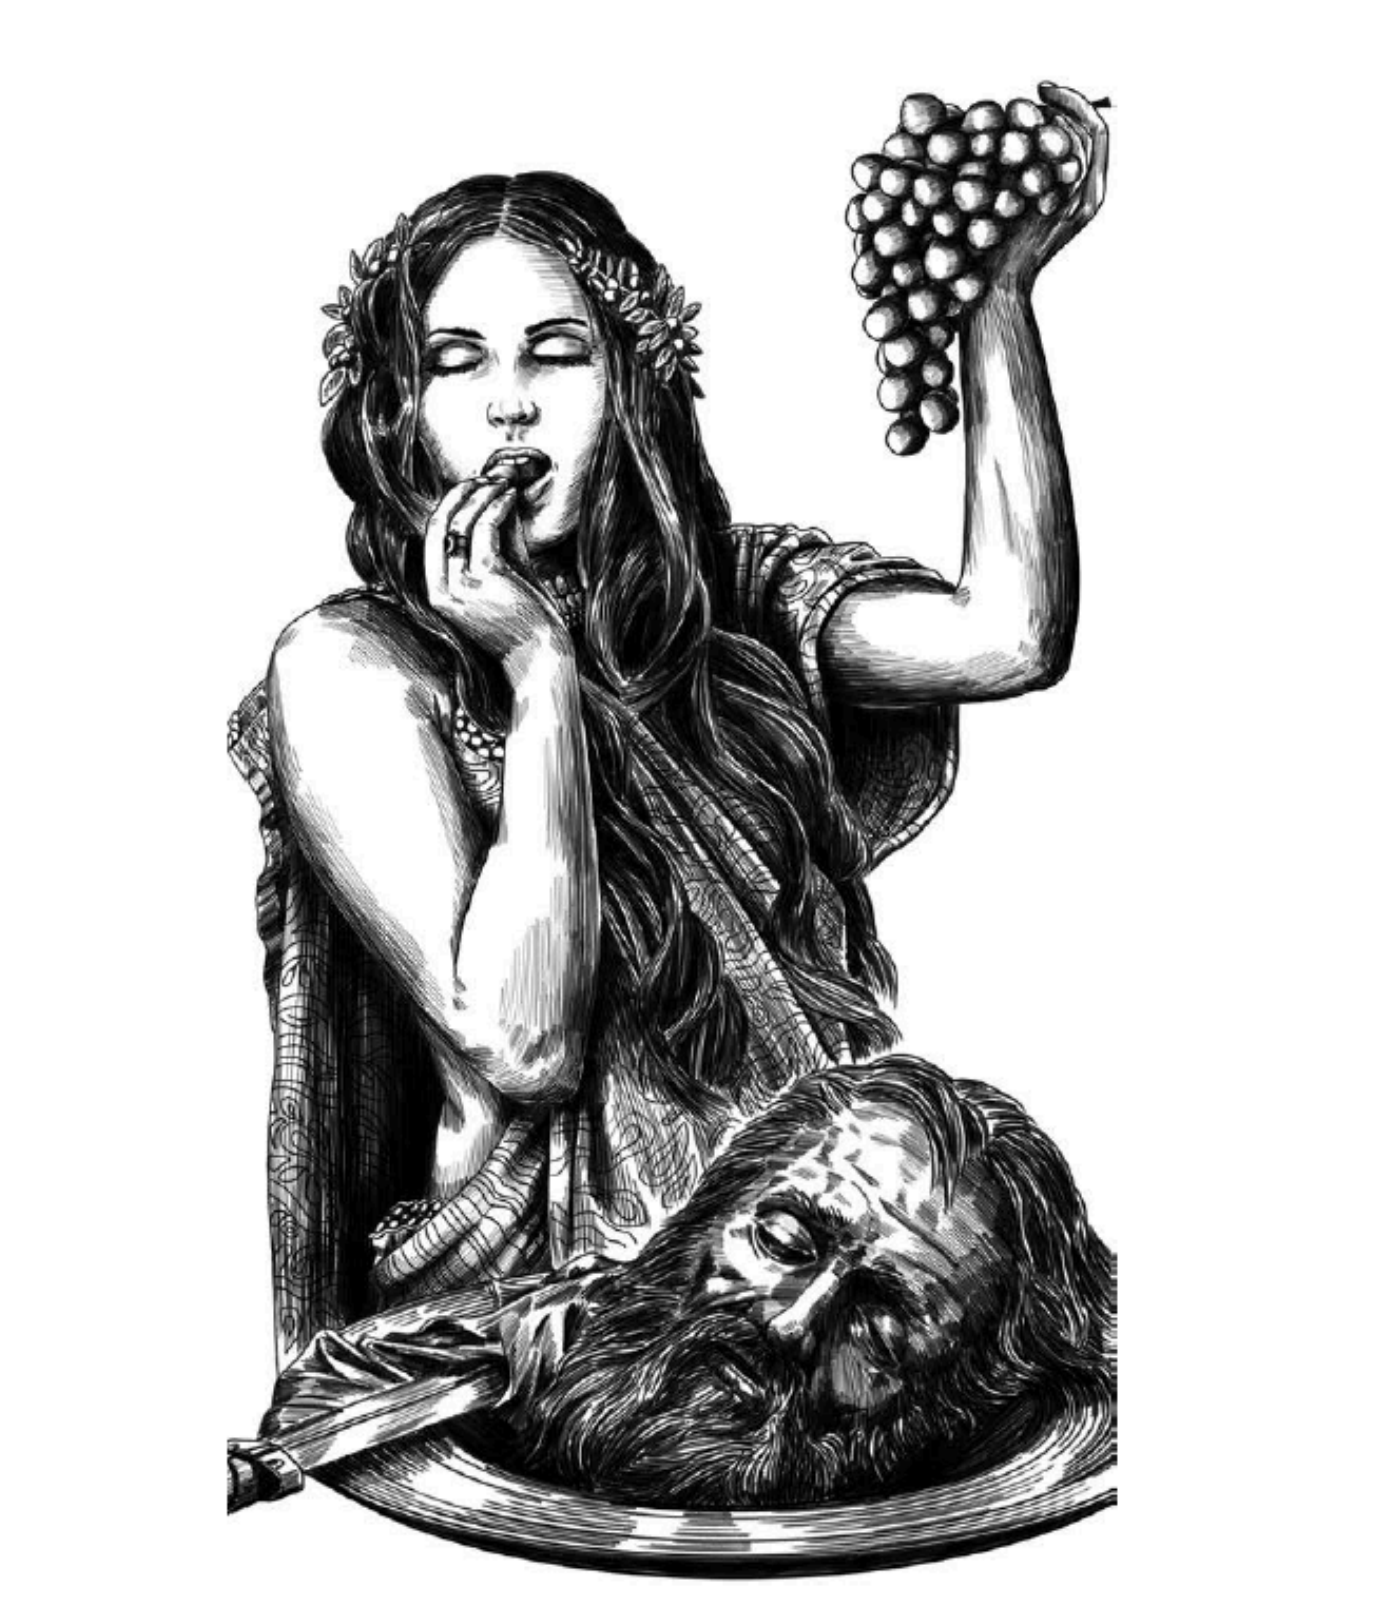
\includegraphics[width=1\textwidth]{assets/john-the-baptist.png}
    \label{fig:john-the-baptist}
\end{figure}

\newpage
First, what was the nature of Herod's previous, dissolved marriage? Let's give the floor to Metropolitan Joseph, commentator on \emph{Antiquities}:

\begin{smallquote}
    With his tetrarchy sharing a border with such longtime predators as the Arabs, Antipas greatly facilitated the security of his subjects by building new military fortifications in the outskirts of the country. And not for nothing is his very marriage to the daughter of the Arabian king Aretas suspected to have been an act of pure political calculation, which would serve to ensure peace for his country better than any fortresses or weaponry could, assuming the marriage was not imposed upon him by Augustus.\footnote{\emph{The History of the Jewish People According to Flavius Josephus' Antiquities}, book III, chapter VII.}
\end{smallquote}
The dissolution of this forced, dynastic marital union---at his wife's initiative, no less---resulted in Herod's ill-fated border war with Aretas, but that's a whole other story.

Second, Herodias was previously the wife of Herod's stepbrother, not his biological one (as is commonly thought); the aforementioned Metropolitan Joseph provides ample evidence for this fact. It's not at all surprising that Josephus' account presents this as a completely ordinary story of a second marriage; in general, the Jews saw marriage not as a sacrament, but as a civil status, so divorce was an extremely common occurrence. I should note that Josephus himself was a member of the Pharisees, who were renowned for their expert knowledge in Mosaic Law; moreover, he had no warm feelings for the hellenized Herod. You would think that he, out of all people, would waste no opportunity to take yet another dig at the worthy offspring of Herod the Bloody---assuming there was anything even remotely criminal about the affair.

Third, Herodias has always been seen as a calculating seductress, who not only broke all laws of marriage just to wrap the king of Galilee around her finger, but then, toying with an ax, kept a watchful eye on her cozy perch by the throne. And again, that doesn't track. Several years later, the emperor Caligula ordered, so to speak, the ``dismissal of Mr. Antipas, Tetrarch of Galilee and Perea, from his present position due to his inability to fulfill his duty,'' and exiled him to Spain, where he ultimately died---in poverty, obscurity, and total isolation. The only person who shared his exile with him, up until his dying day, was Herodias. It makes me wonder: would a woman like that really care what some scruffy, unwashed puritan was shouting about her ``family values''?

And now, the actual episode of John's beheading. Let's start off with a seemingly basic question: where did it take place? Well, the king is celebrating his birthday with his courtiers, military commanders, and elders; in light of the absence of any specific indications in the text, it would be logical to assume that the feast was held at its typical location---Herod's palace at Tiberias, on the Sea of Galilee. But during that time, John was held captive at the fortress of Machaerus (or Macheron), which is on the Dead Sea---and this comes from the same testimony by Josephus that the Church takes as fact! It should be noted that the Evangelists' account states that Herod did not merely give the order to execute John the Baptist (for which purpose he could have sent messengers from Tiberias to Machaerus, about 60 kilometers as the crow flies); no, right then and there, after several minutes had passed, he presented his stepdaughter the platter with the prophet's severed head.

In trying to resolve this obvious contradiction, some Christian commentators have tried---completely arbitrarily---to move the scene's location to Machaerus (if the mountain won't come to Muhammad, then Muhammad must go to the mountain). Gladkov, for example, goes so far as to tie this to political events:

\begin{smallquote}
    Insulted [due to his daughter's divorce---K.E.], Aretas started a war against Herod; as a consequence of this, Herod and his entire court moved to Machaerus, where he had imprisoned John the Baptist, and took up residency in his palace there.
\end{smallquote}
Well, let's start with the fact that Macherus was a small border outpost in the outskirts of the Arabian desert, and needless to say, there were no palaces there to speak of. Only recently, at the start of the protracted border war between Herod and Aretas, had the Jews captured the fortress from the Arabs, who had controlled it in previous years. Pretty strange idea to go to a place like that for your birthday, don't you think? Not to mention---what king brings his entire court, including his wife and children, out to an \emph{active war zone}?

Or consider this detail: after Herod's ill-advised promise, Salome ``went out and said to her mother, `What shall I ask?' And she said, `The head of John the Baptist!' Immediately she came in with haste to the king and asked, saying, `I want you to give me at once the head of John the Baptist on a platter''' (Mk 6:24-25). Well, I'll be... I guess the princess put on a striptease for her stepfather's drunken guests just for the hell of it, with no concrete goal in mind beforehand?

For these reasons, I cannot help but be extremely skeptical of the Evangelists' version of the events. From an artistic perspective, though, the story is truly magnificent. It manages to organically combine obvious folklore elements (``Even if you ask for half my kingdom!'') with a tightly structured plot---and just by itself, the semantic hieroglyph of the ``head on a platter'' provides ample fodder for pretentious art critics and psychoanalysts! Of course, to preserve the dynamism of the action (the immediate fulfillment of Herod's rash promise), it was necessary to sacrifice some degree of accuracy and move John to Tiberias (or alternatively, Herod to Machaerus), but such a sacrifice seems fully justified. It seems highly improbable that such a plot could spontaneously ``clump together'' from the various rumors circulating about the death of the popular prophet.

All of this allows me to make the following conjecture: this rumor about the circumstances of John the Baptist's demise, which the Evangelists Mark and Matthew faithfully reproduced in their respective Gospels, was the result of an ``active measures'' campaign.\footnote{A contemporary term referring to the practice of influencing public opinion through channels of official propaganda. A classical example of ``active measures'' is described in Leonid Solovyov's \emph{The Tale of Hodja Nasreddin}, where undercover guards in teahouses and caravanserais try to convince the people of Bukhara that their beloved Hodja has been a longtime servant of the emir. A more recent example is the use of KGB-controlled newspapers (mainly in third-world countries) to disseminate stories claiming that the AIDS virus was created in a Pentagon laboratory (see \emph{KGB: The Inside Story of Its Foreign Operations from Lenin to Gorbachev} by Christopher Andrew and Oleg Gordievsky, pp. 529-530). (K.E.)} Its goal seems quite obvious: to shift a significant portion of the blame away from Herod (who supposedly ``did many things when he heard John, and heard him gladly''), depicting the tetrarch as the naive victim of perennial feminine guile. Who, then, was the initiator of this (judging from its result) exceptionally competent campaign to shape the public opinion of Palestine?

The answer, as I see it, will emerge of its own accord when we can successfully answer another question, closely tied to the first: who arrested John the Baptist? Right now, the reader is probably looking at me like I'm a total idiot---after all, the Evangelists and Josephus seem to be in complete agreement on this point. So let me refine the question a little: let's suppose it really was Herod who \emph{executed} John. But who \emph{carried out the arrest}, and on what grounds? The Gospel texts lack any concrete indications in this regard; what's more, the situation here is nowhere near as simple as it first appears, and here's why.

The problem is that John was a native of Judea, and lived there his whole life. He led an ascetic existence preaching in the Judean desert and the Jordan River Valley near Bethabara and Aenon. At times, he would travel to the left bank of the Jordan in Perea, but by all accounts, he never spent any time in Galilee. Therefore, John's preaching should really have only been a headache for the Judean high priests and procurator---not Herod. Moreover, the Judean leadership was actually quite sympathetic to the prophet (at least in the beginning), and many Pharisees and Sadducees even sought to be baptized by him (Mt 3:7).

Furthermore, if the tetrarch of Galilee wanted to get his hands on the scandalous preacher, it wouldn't be too easy to do; Judea was in at least some sense a foreign country, and the relationship between the Judean and Galilean authorities left much to be desired. But perhaps John, for reasons unknown to us, left Herod so upset by his preaching that he decided to thumb his nose at both the law and common courtesy, and send an arrest team into foreign territory?\footnote{Anyone who believes that the extraterritorial ``actions'' of the NKVD, whose victims included Alexander Kutepov, Leon Trotsky, and countless other Russian emigres, were an unprecedented event in world history, is sorely mistaken. The secret services of civilized and democratic France, for example, took great pleasure in kidnapping and killing OAS agents who had fled across the border, paying no heed to the protests of their neighbors---carrying on a proud tradition that started with the abduction of the Duke of Enghien by Napoleon's gendarmes. (K.E.)}

While we can't rule out this possibility, it would render Christ's reaction to this event utterly incomprehensible, considering that he was also in Judea at the time: ``Now when Jesus heard that John had been put in prison, He departed \emph{to Galilee}'' (Mt 4:12).

So, let's try to sum up everything we've established so far. First, a rather popular and influential spiritual leader was preaching in Palestine at the same time as Jesus Christ. Second, his relationship to the Son of Man was apparently not as idyllic as is commonly believed. Third, the death of said leader took place in highly unclear circumstances, the nature of which I suggest we ought to reflect on.